%\begin{frame}
%\frametitle{A quasi-hierarchy of algebraic theories}
%	\begin{description}
%		\pause \item[Theory] :: domain of discourse
%		\pause \item[Elementary Algebra] :: equational reasoning in a particular algebra
%		\pause \item[Abstract Algebra] :: particular classes of algebras such as groups, rings, or fields
%		\pause \item[Universal algebra] :: classes of classes of algebras
%		\pause \item[Category theory] :: given a list of operations and axioms in universal algebra the corresponding algebras and homomorphisms between them can represent objects and morphisms in a category
%	\end{description}
%\end{frame}

\subsection{functor categories}

\begin{frame}
\begin{figure}
\noindent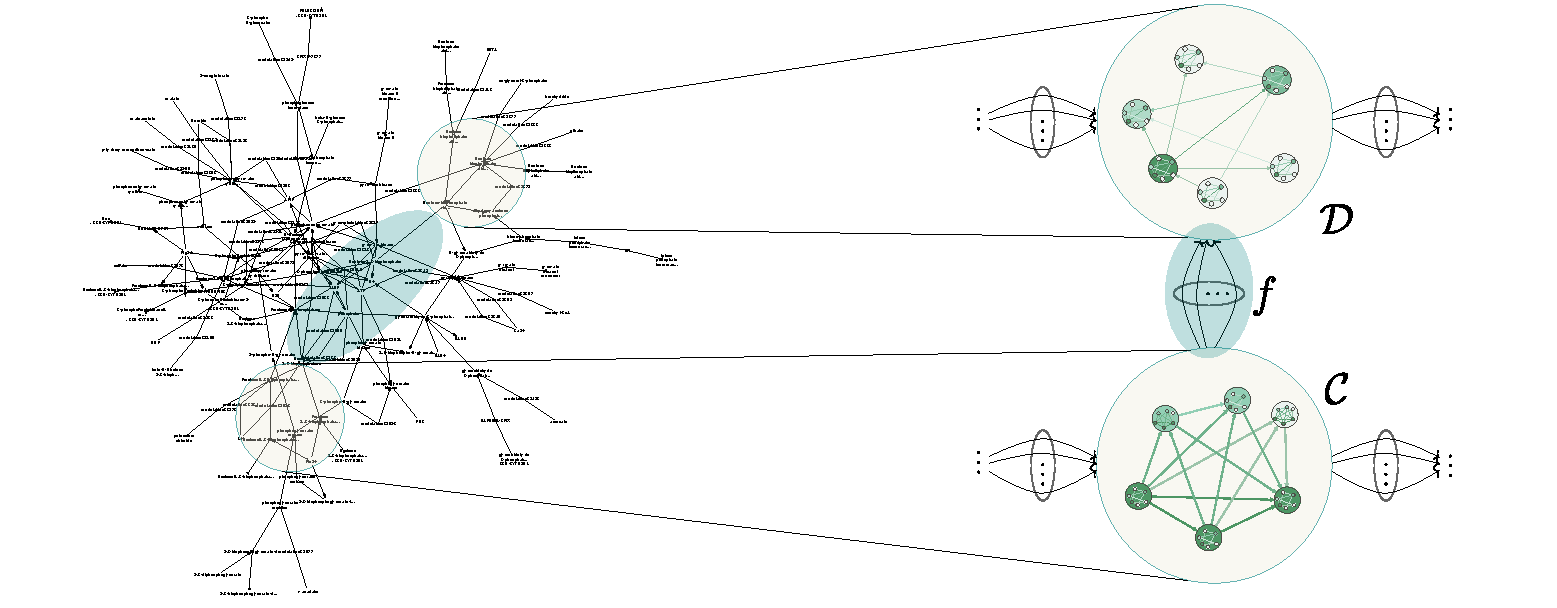
\includegraphics[width=1.0\framewidth]{fig/biograph.pdf}
\caption{
%Particular features of interaction networks underlying biological systems can be abstracted as algebraic structures of some type with morphisms translating structure between them.
On the left is a representation of the integrated metabolic-gene regulatory glycolytic network of E. coli K12 MG1655 derived from the EcoCyc database \cite{Keseler2011} in terms of the BioPAX ontology \cite{Demir2010}.
%On the right is a conceptual picture of the way in which the relationships between substructure of a particular network can be represented algebraically in terms of algebraic structures that can be referred to as objects and methods of transforming or mapping between these structures referred to as morphisms.}
}
\label{fig:biograph}
\end{figure}
\end{frame}

\begin{frame}
We can define a category having functors as objects and natural transformations as morphisms, which is called a functor category, by recognizing that every functor $F$ comes with the {\it identity} transformation $\text{id}_F : F \to F$. In addition, given a morphism of
functors $t : F \to G$ and a morphism of functors $s : E \to F$
then the {\it composition} $t \circ s$ is defined by the rule
$$
(t \circ s)_x = t_x \circ s_x : E(x) \to G(x)
$$
for $x \in \Ob(\mathcal{A})$.
This is a morphism of functors
from $E$ to $G$.
Thus, given categories
$\mathcal{A}$ and $\mathcal{B}$ we obtain the category of functors between $\mathcal{A}$ and
$\mathcal{B}$.
\end{frame}

\begin{frame}
\iftoggle{thmsty}{
\begin{definition}
\label{definition-equivalence-categories}
}{}
An {\it equivalence of categories}
$F : \mathcal{A} \to \mathcal{B}$ is a functor such that there
exists a functor $G : \mathcal{B} \to \mathcal{A}$ such that
the compositions $F \circ G$ and $G \circ F$ are isomorphic to the
identity functors $\text{id}_\mathcal{B}$,
respectively $\text{id}_\mathcal{A}$.
In this case we say that $G$ is a {\it quasi-inverse} to $F$.
\iftoggle{thmsty}{
\end{definition}
}
\end{frame}

\subsection{adjoint functors}

\begin{frame}
\iftoggle{thmsty}{
\begin{definition}
\label{definition-adjoint}
}{}
Let $\mathcal{C}$, $\mathcal{D}$ be categories.
Let $u : \mathcal{C} \to \mathcal{D}$ and
$v : \mathcal{D} \to \mathcal{C}$ be functors.
We say that $u$ is a {\it left adjoint} of $v$ or that
$v$ is a {\it right adjoint} to $u$, written $u \dashv v$, if there are bijections
$$
\phi_{X,Y}:\Mor_\mathcal{D}(u(X), Y)
\simeq
\Mor_\mathcal{C}(X, v(Y))
$$
functorial in $X \in \Ob(\mathcal{C})$, and
$Y \in \Ob(\mathcal{D})$.
\iftoggle{thmsty}{
\end{definition}
}
\end{frame}

\begin{frame}
$F \dashv G$ is thus equivalent to the statement $\phi_{-,-}:b_{(-)} \cong b^{(-)}$. In this framework, information encoding/decoding is an asymmetric process that can only be accomplished without loss of information in one direction: objects of $\mathcal{D}$ can be encoded into objects of $\cC$ and decoded into objects of $\mathcal{D}$ but, in general, proceeding in the opposite order may result in loss of information. This asymmetry is clarified by consideration of the unit and counit morphisms of the adjunction.
\end{frame}

\begin{frame}
\iftoggle{thmsty}{
\begin{definition}
\label{definition-unit}
}{}
Consider the identity morphism $1_{Fc} \in \Mor_{\mathcal{D}}(Fc,Fc)$. The adjoint transpose of $1_{Fc}$ is the {\it unit} morphism at $c$
$$
\phi_{c,Fc}(1_{Fc})=1_{Fc}^*=\eta_c: c \rightarrow GFc
$$
where $\eta_c \in \Mor_{\cC^{opp}}(c,GFc)$, which, when taken to be natural in $c \in \Ob(\cC^{opp})$, gives the natural transformation
$$
\eta : 1_{\cC^{opp}} \Rightarrow GF
$$
\iftoggle{thmsty}{
\end{definition}
}
\end{frame}

\begin{frame}
\iftoggle{thmsty}{
\begin{definition}
\label{definition-counit}
}{}
Consider the identity morphism $1_{Gd} \in \Mor_{\cC^{opp}}(Gd,Gd)$. The adjoint transpose of $1_{Gd}$ is the {\it counit} morphism at $d$
$$
\phi_{Gd,d}^{-1}(1_{Gd})=1_{Gd}^*=\epsilon_d: FGd \rightarrow d
$$
where $\epsilon_d \in \Mor_{\mathcal{D}}(d,FGd)$, which, when natural in $d$, gives the natural transformation
$$
\epsilon: FG \Rightarrow 1_{\mathcal{D}}
$$
\iftoggle{thmsty}{
\end{definition}
}
\end{frame}

\begin{frame}
The adjoint relationship between functors $F \dashv G$ with unit $\eta$ and counit $\epsilon$ natural transformations. The asymmetry in the encoding-decoding relationship indicates that $FG \mathcal{D}$ can be translated back into the original terms of $\mathcal{D}$ whereas $GF \cC^{opp}$ cannot necessarily be translated back into the original terms of $\cC^{opp}$.
\begin{center}
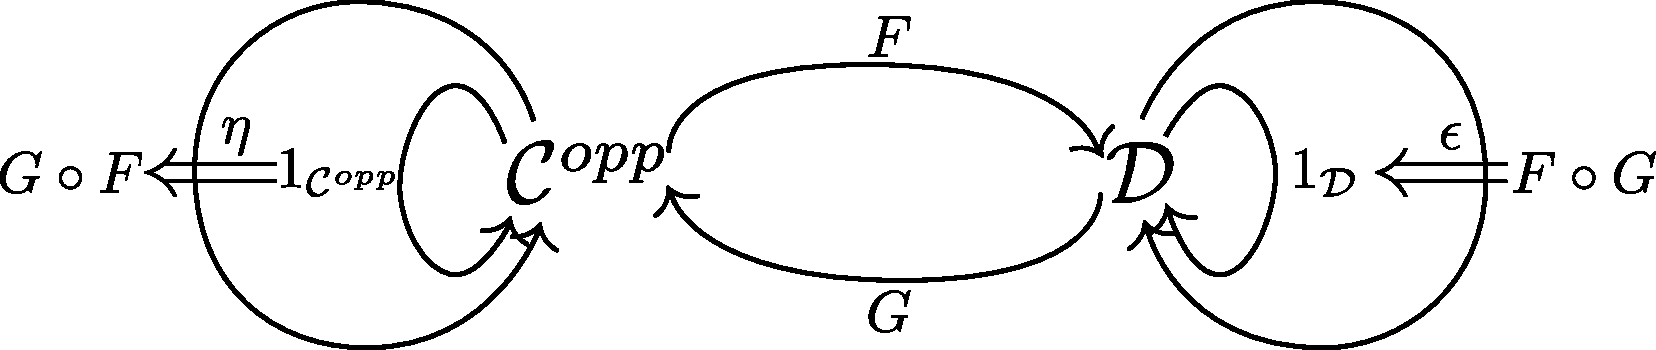
\includegraphics[width=0.9\framewidth]{fig/adjunction.pdf}
\end{center}
\end{frame}

\subsection{encoding and decoding}
\begin{frame}
The composite encoding inspection functor 
$$
b_{(-)} \circ G(-): \mathcal{D} \rightarrow \cC^{opp} \rightarrow \textit{Sets}
$$
that specifies a set of morphisms in $\mcD$ from the perspective of $\cC^{opp}$ is represented by the pair $(F,\eta)$. Likewise, the composite decoding inspection functor 
$$
b^{(-)} \circ F(-): \cC^{opp} \rightarrow \mcD \rightarrow \textit{Sets}
$$
that specifies a set of morphisms in $\cC^{opp}$ from the perspective of $\mcD$ is represented by the pair $(G,\epsilon)$.
\end{frame}

\begin{frame}
The asymmetry of the adjunction can be dispensed with if the unit and counit natural transformations are in fact natural isomorphisms $\eta: 1_{\cC^{opp}} \cong GF$ and $\epsilon: FG \cong 1_{\mcD}$. In any limit in which this is the case the adjunction $F \dashv G$ gives an equivalence of categories $\cC^{opp} = \mcD$ and the information encoding-decoding process becomes bidirectionally exact.
\end{frame}